\section{Strömungslinien}
\label{joukowski:sec:stroemungslinien}
	\subsection{Allgemeine Definition}
		Um ein Verständnis dafür aufzubauen, wie die Luft um ein Flügelprofil strömt,
		muss zunächst ein grundlegendes mathematisches Verständnis einer Strömung,
		sowie ihres Geschwindigkeitsvektorfeldes vorhanden sein.
		In diesem Abschnitt liegt der Fokus darauf,
		das Verständnis von Strömungen zu festigen
		und deren mathematischen Beschreibung in der komplexen Ebene aufzuzeigen.
		
		Unsere komplexe Strömungsfunktion kann als
		\[
			f(z)
			= 
			\phi(z) + i \psi(z)
		\]
		geschrieben werden.
		Punkte in der $z$-Ebene, für welche $\phi(z)$ einer Konstanten entsprechen, werden \emph{Äquipotentiallinien} genannt
		und Punkte, für welche $\psi(z)$ einer Konstanten entsprechen, werden \emph{Strömungslinien} genannt.
		Für unsere Betrachtungen sind die Strömungslinien von grosser Bedeutung.
		
		\begin{definition}[Strömungslinie]
			\label{joukowski:stroemungslinien:proof:Stroemungslinie}
			In der \emph{stationären Strömung} beschreibt eine \emph{Strömungslinie} den Weg, welcher ein Luft- oder Fluidteilchen nimmt
			und gilt für alle Punkte $z$ die
			\[
				\psi(z) = C
			\]
			erfüllen.
			Wobei unterschiedliche Konstanten $C$ unterschiedliche Strömungslinien bezeichnen.
		\end{definition}
		Um die Strömungslinien übersichtlich darzustellen, stehen nur eine diskrete Anzahl Konstanten $C$ aus der Definition~\ref{joukowski:stroemungslinien:proof:Stroemungslinie} zur verfügung.
		
		\begin{beispiel}
			\label{joukowski:stroemungslinien:beispiel:ungestoerte-Stroemung}
			Beginnen wir mit einer möglichst einfachen Strömung: Eine, welche homogen ungehindert von links nach rechts strömen kann.
			Es wird sofort deutlich, dass die Strömungslinien horizontal verlaufen und vertikal gleichmässig verteilt sind.
			Somit ist die Geschwindigkeit an jedem Punkt des Raumes identisch.
			Die Abbildung~\ref{joukowski:Stroemungslinien:fig_Allgemein}, welche dieser Situation entspricht,
			kann mit der Strömungsfunktion $f(z) = z$ und ${v(z)} = 1$ beschrieben werden.
		\end{beispiel}
		
		\begin{figure}

	\centering
	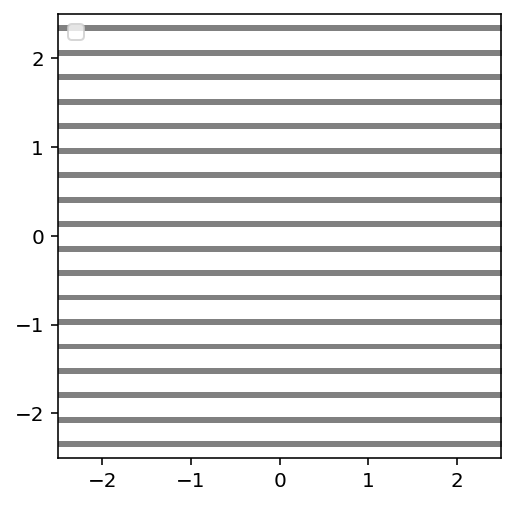
\includegraphics[width=0.45\textwidth]{papers/joukowski/images/05_stroemungslinien/Strom_g.png}
	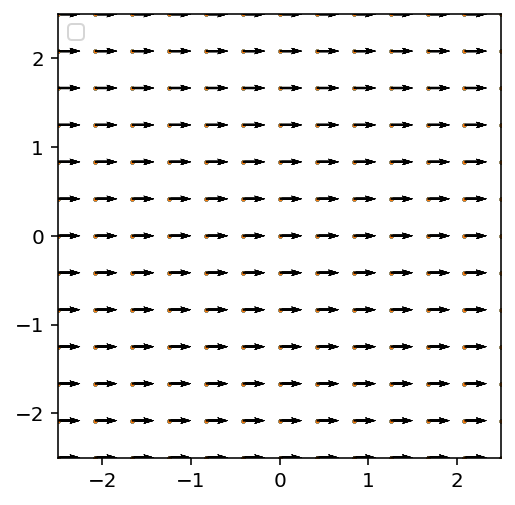
\includegraphics[width=0.45\textwidth]{papers/joukowski/images/05_stroemungslinien/speed.png}
	\caption{
		Für die homogene Strömung $f(z) = z$ sind die Strömungslinen horizontal
		und das Geschwindigkeitsvektorfeld $v(z)$ ist konstant.
		\label{joukowski:Stroemungslinien:fig_Allgemein}
	}
\end{figure}

		\begin{figure}

	\centering
	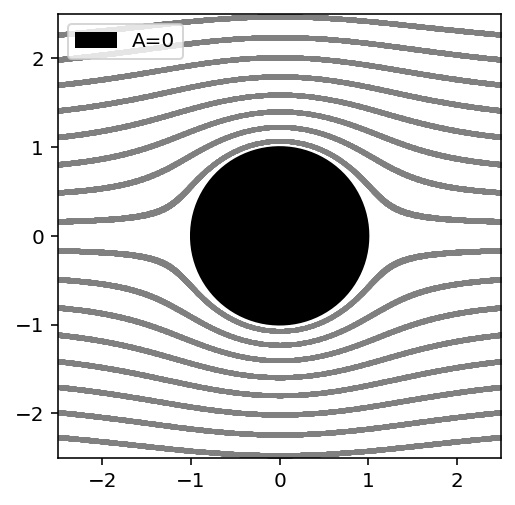
\includegraphics[width=0.45\textwidth]{papers/joukowski/images/05_stroemungslinien/Magnus_Strom_A000_g.png}
	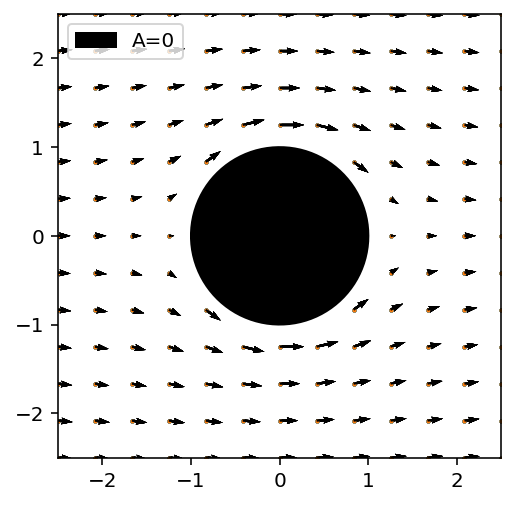
\includegraphics[width = 0.45\textwidth]{papers/joukowski/images/05_stroemungslinien/Magnus_Speed_A000.png}
	\caption{
		Die Strömungslinien werden lokal um das Hindernis des Zylinders gekrümmt,
		dabei nimmt die Geschwindigkeit der Strömung ober- und unterhalb des Zylinders gleichmässig zu.
		\label{joukowski:Stroemungslinien:fig_Zylinder}
	}
\end{figure}

		
		\begin{beispiel}
		\label{joukowski:stroemungslinien:beispiel:joukowski-transformation}
		In einem zweiten Beispiel fügen wir einen Zylinder als Hindernis ein.
		Um diese Situation zu analysieren, müssen wir eine komplexe Funktion finden, welche unser Hindernis auf eine horizontale Linie abbildet.
		Finden wir diese Funktion,
		so bildet diese auch die Strömungslinien auf die horizontalen Strömungslinien aus Beispiel~\ref{joukowski:stroemungslinien:beispiel:ungestoerte-Stroemung} ab.
		
		Diese Eigenschaft gilt nur,
		wenn diese Funktion \emph{biholomorph} ist.
		
		\begin{definition}[Biholomorphe Funktion]
			Eine komplexe Funktion $f(z)$ ist biholomorph, wenn
			\begin{enumerate}
				\item $f(z)$ holomorph ist
				und
				\item ihre Umkehrfunktion $f^{-1}(z)$ auch holomorph ist.
			\end{enumerate}
		\end{definition}
		
		Die Funktion, welche einen Kreis auf eine horizontale Linie abbildet, ist die sogenannte Kutta-Joukowski-Transformation und lautet
		\begin{equation}
			\label{joukowski:Stroemungslinien:equation_zylinder}
			f(z)
			=
			\frac{v_\infty}{2} \cdot \biggl(z+\frac{1}{z}\biggr).
		\end{equation}
		%TODO wieso /2, sollte es nicht einfach v_infty sein?
		Die Ableitung dieser Funktion nach $z$ entspricht dann
		\begin{equation}
			\label{joukowski:Stroemungslinien:equation_zylinder_speed}
			\frac{df}{dz}
			=
			\overline{v(z)}
			=
			\frac{v_\infty}{2} \cdot \biggl(1 - \frac{1}{z^2}\biggr).
		\end{equation} 
		Die Strömungslinien dieser Funktion sowie die Geschwindigkeit werden in Abbildung ~\ref{joukowski:Stroemungslinien:fig_Zylinder} dargestellt.
		\end{beispiel}
		
	\subsection{Zusammenhang zwischen $f(z)$ und $\overline{v(z)}$}
		\label{joukowski:stroemungslinien:zusammenhang-fz-z}
		In Beispiel~\ref{joukowski:stroemungslinien:beispiel:joukowski-transformation}
		haben wir geschrieben
		\[
			\frac{df}{dz}
			=
			\overline{v(z)}.
		\]
		Dies scheint auf den ersten Blick etwas merkwürdig zu sein,
		da im Reelen die Ableitung direkt die Geschwindigkeit selbst gibt.
		Dieses Resultat stammt aus den Cauchy-Riemann-Differentialgleichungen und der Konvention, die komplexe Geschwindigkeit als $u+iw$ zu schreiben.
		
		\begin{proof}
			\label{joukowski:stroemungslinien:v-konjugiert-komplex}
			Wir berechnen die komplexe Ableitung der Funktion $f(z)$ nach $z$.
			Als erstes teilen wir $f(z)$ in Real- und Imaginärteil und schreiben
			\[
				\frac{df}{dz}
				=
				\frac{d\phi}{dz} + i \frac{d\psi}{dz}.
			\]
			Jetzt können wir ausnutzen, dass es bei einer holomorphen Funktion keine Rolle spielt in welche Richtung die Ableitung erfolgt,
			was heisst, dass
			\[
				\frac{df}{dz}
				=
				\frac{df}{dx}
				=
				\frac{df}{idy}
			\]
			gilt.
			Dabei nutzen wir aus den Cauchy-Riemann-Differentialgleichungen die Zusammenhänge
			\[
				\frac{d\phi}{dz}
				=
				\frac{\partial \phi}{\partial x}
				\qquad
				\text{und}
				\qquad
				\frac{d\psi}{dz}
				=
				-\frac{\partial \phi}{\partial y}
			\]
			ein.
			Es ist eine Konvention
			\[
				u
				=
				\frac{\partial \phi}{\partial x}
				\qquad
				\text{und}
				\qquad
				w
				=
				\frac{\partial \phi}{\partial y}
			\]
			zu schreiben.
			Somit ergibt sich schliesslich
			\[
				\frac{df}{dz}
				=
				u - iw
				=
				\overline{v(z)}.
			\]
		\end{proof}
	